\documentclass[10pt, conference, letterpaper]
{IEEEtran}

\usepackage{algorithm}
\usepackage{algorithmicx}
\usepackage{algpseudocode}
\usepackage{amsfonts}
\usepackage{amsmath}
\usepackage{amssymb}
\usepackage[ansinew]{inputenc} 
\usepackage{xcolor}
\usepackage{mathtools}
\usepackage{graphicx}
\usepackage{caption}
\usepackage{subcaption}
\usepackage{import}
\usepackage{multirow}
\usepackage{cite}
\usepackage[export]{adjustbox}
\usepackage{breqn}
\usepackage{mathrsfs}
\usepackage{acronym}
%\usepackage[keeplastbox]{flushend}
\usepackage{setspace}
\usepackage{bm}
\usepackage{stackengine}
\usepackage{float}
\usepackage{listings}
\usepackage{url}


\lstset{%
 backgroundcolor=\color[gray]{.85},
 basicstyle=\small\ttfamily,
 breaklines = true,
 keywordstyle=\color{red!75},
 columns=fullflexible,
}%

\lstdefinelanguage{BibTeX}
  {keywords={%
      @article,@book,@collectedbook,@conference,@electronic,@ieeetranbstctl,%
      @inbook,@incollectedbook,@incollection,@injournal,@inproceedings,%
      @manual,@mastersthesis,@misc,@patent,@periodical,@phdthesis,@preamble,%
      @proceedings,@standard,@string,@techreport,@unpublished%
      },
   comment=[l][\itshape]{@comment},
   sensitive=false,
  }

\usepackage{listings}

% listings settings from classicthesis package by
% Andr\'{e} Miede
\lstset{language=[LaTeX]Tex,%C++,
    keywordstyle=\color{RoyalBlue},%\bfseries,
    basicstyle=\small\ttfamily,
    %identifierstyle=\color{NavyBlue},
    commentstyle=\color{Green}\ttfamily,
    stringstyle=\rmfamily,
    numbers=none,%left,%
    numberstyle=\scriptsize,%\tiny
    stepnumber=5,
    numbersep=8pt,
    showstringspaces=false,
    breaklines=true,
    frameround=ftff,
    frame=single
    %frame=L
}

\renewcommand{\thetable}{\arabic{table}}
\renewcommand{\thesubtable}{\alph{subtable}}

\DeclareMathOperator*{\argmin}{arg\,min}
\DeclareMathOperator*{\argmax}{arg\,max}

\def\delequal{\mathrel{\ensurestackMath{\stackon[1pt]{=}{\scriptscriptstyle\Delta}}}}

\graphicspath{{./figures/}}
\setlength{\belowcaptionskip}{0mm}
\setlength{\textfloatsep}{8pt}

\newcommand{\eq}[1]{Eq.~\eqref{#1}}
\newcommand{\fig}[1]{Fig.~\ref{#1}}
\newcommand{\tab}[1]{Tab.~\ref{#1}}
\newcommand{\secref}[1]{Section~\ref{#1}}

\newcommand\MR[1]{\textcolor{blue}{#1}}
\newcommand\red[1]{\textcolor{red}{#1}}
\newcommand{\mytexttilde}{{\raise.17ex\hbox{$\scriptstyle\mathtt{\sim}$}}}

%\renewcommand{\baselinestretch}{0.98}
% \renewcommand{\bottomfraction}{0.8}
% \setlength{\abovecaptionskip}{0pt}
\setlength{\columnsep}{0.2in}

% \IEEEoverridecommandlockouts\IEEEpubid{\makebox[\columnwidth]{PUT COPYRIGHT NOTICE HERE \hfill} \hspace{\columnsep}\makebox[\columnwidth]{ }} 

\title{Lightweight keyword spotting using attention-based recurrent neural networks}

\author{Matteo Moratello$^\dag$, Enrico Petrucci$^\ddag$
\thanks{$^\dag$Department of Information Engineering, University of Padova, email: moratellom@dei.unipd.it}
\thanks{$^\ddag$Department of Information Engineering, University of Padova, email: petruccien@dei.unipd.it}
} 

\IEEEoverridecommandlockouts

\newcounter{remark}[section]
\newenvironment{remark}[1][]{\refstepcounter{remark}\par\medskip
   \textbf{Remark~\thesection.\theremark. #1} \rmfamily}{\medskip}

\begin{document}

\maketitle

\begin{abstract}
The problem of Keyword spotting (KWS) has been gaining relevance in recent years due to the increasing diffusion of voice controlled devices. These kinds of devices require high accuracy models, in order to be reliable enough, but with a small footprint since their limited power consumption and hardware capabilities.
In this paper we investigate two learning architectures, namely recurrent neural networks that use the attention mechanism, and residual neural networks to address this problem and propose new models.
Our best recurrent neural networks can outperform the previous state-of-the-art models while having less parameters. The most accurate model that we found has an accuracy of 97.1\% while having 155K parameters.  We also present a lightweight model that has only  25K parameters, a fraction of the usual amount, but manages to perform comparably and sometimes even better than larger models in the literature, managing to reach an accuracy of 96.6\%.
Even our res-net models managed to surpass, in terms of performance, the previous models that were based on this kind of architecture. We show detailed comparisons between our new models and the best models in previous literature.
These kinds of high accuracy, but small-footprint models are crucial for delivering less expensive and reliable devices.\\ 
\end{abstract}

\IEEEkeywords
Command Recognition, Keyword Spotting, Recurrent Neural Network, Residual Neural Network, Attention
\endIEEEkeywords


% !TEX root = template.tex

\section{Introduction}
\label{sec:introduction}

In recent years, the diffusion of devices that rely on keyword spotting to start interactions has been steadily expanding. These kinds of devices that can be voice-activated and voice-controlled are increasingly common and more than ever part of our lives, from the phones inside our pockets and the watches on our wrists to the smart home devices (like Google Home or Amazon Echo), or even industrial equipment.
These systems are often connected to a powerful server that performs the heavy-duty computations like actual speech recognition. However, relying only on the remote processing power would imply transmitting a considerable amount of recordings over the web that isn't scalable and poses a problem for security and privacy.


A possible solution is equipping these local devices with modules that can locally perform a keyword spotting task that eventually triggers the communication with the web service.
These models need to be small and computationally light to be as energy-efficient as possible in order to run in battery-powered devices and with limited computational and cooling capabilities.
The development of such speech command recognition models can be useful also for other applications in which the internet coverage is not available.
This problem has already been addressed in the literature and the state-of-the-art results are presented in the papers \cite{1} \cite{2}, where small-footprint models are described. In \cite{1} the model presented is based on recurrent neural networks - that make use of the attention mechanism - and on residual networks. It was shown that using those kinds of architectures was possible to largely improve upon previous CNN models \cite{3}, both for accuracy and number of parameters. The results presented in these papers, especially in \cite{2}, show that the accuracy of their models suffered significantly when decreasing the number of parameters.


In this work we present and compare different models -- that perform the keyword spotting task -- improving on the state of the art tradeoff between high accuracy and small footprint, exploring possible solutions by adopting both recurrent neural networks based on the attention mechanism and residual neural networks. A decrease in the model footprint could sensibly reduce hardware requirements, meaning fewer production costs that can imply lower retailing prices, and possibly less power consumption in battery-powered devices.


In this paper we will introduce:
\begin{itemize}
  \item an attention-based recurrent neural network that slightly improves the accuracy with respect to the best performing model in the literature, while having a smaller footprint; 

  \item another model that, with 8 times fewer parameters than the previous best performing model, but can still achieve high accuracy of 96.6%;
  \item improved models based on the residual network architecture improving on the previously available tradeoff for this kind of model.

\end{itemize}


The remainder of the paper is organized as follows. In Section II we describe the state of the art; the system and data models are respectively presented in Sections III and IV. The proposed learning models are detailed in Section V and their evaluation is carried out in Section VI.
Concluding remarks are provided in Section VII.


% !TEX root = template.tex

\section{Related Work}
\label{sec:related_work}

In the literature the use of neural networks for solving the \textit{keyword spotting} problem -- that consists in the identification of speech commands -- is not new and this allows us to have a good reference point in terms of both accuracy and model dimension for different architectures. In \cite{4}, where the dataset that we used is presented, along with the instructions on how to perform training and testing, there is also a baseline for the accuracy in the test set by a simple model that consists of a convolutional neural network inspired by \cite{10}. In \cite{3} they improved the convolutional neural networks models, comparing straiding and pooling both in time and frequency in order to reduce the number of parameters and multiplications. Moreover, they have shown the advantages of using CNN as opposed to DNN.


A greater improvement from simple CNNs has been seen in \cite{2}, where \textit{residual neural networks} are explored with relative success. In that paper are presented both wide models which obtain high accuracy, and narrow models that are only a fraction of the former, but inevitably pay a small degradation in terms of performance.
All models proposed are characterized by several convolution blocks, each composed of two layers, and where the input of that block is added to its output. These kinds of networks are capable of learning very complex functions avoiding the problem of vanishing gradients, typical of very deep networks. The authors tried to contain the number of parameters of models: by limiting the number of convolution residual blocks, using convolution dilation, and implementing average pooling layers in order to reduce the input size.
They also used a Reduce Mean layer just before the Dense layer, computing only one value for each feature matrix, this technique is very useful to reduce the number of parameters in the final fully connected layer and we noticed that it works well as regularization.


In \cite{1} the approach used is the one of \textit{recurrent neural networks} based on the \textit{attention mechanism} that, to the best of our knowledge, is the model that obtains the highest accuracy, while having a reasonably small number of parameters. The model they proposed uses, after some convolutions, two bidirectional LSTM layers to extract the long-term dependencies and deploys the attention mechanism to identify the regions containing the most relevant information. The final classification is performed by using dense layers.


Attention-based recurrent neural networks \cite{11, 12} have been able to improve the performance on multiple tasks, mostly in sequence to sequence problems, but had some success even in classification tasks. The advantage of these kinds of models is the fact that different parts of the input are considered with a different magnitude: greater focus is reserved to the most relevant parts of the input.


Deep residual neural networks (ResNets) \cite{9} represent a groundbreaking advance in deep learning that allows us to successfully train very deep networks.
Prior to ResNets, training very deep neural networks was difficult due to the problem of vanishing gradients: as the gradient is back-propagated to earlier layers, repeated multiplication may make the gradient extremely small.
As a result, the performance of the neural network decreases as the network becomes deeper.
ResNets introduced the concept of skip connection.  In common CNNs, we stack more convolutional layers one after the other. With skip connection, we also add the original input to the output of the convolutional block, that is, two or more convolutional layers stacked one after another.
This technique helps to alleviate the vanishing gradients phenomenon and, allowing the model to learn an identity function, ensures that the higher layer will perform at least as good as the lower layer, and not worse.
ResNets were first applied to image recognition, where they contributed to a significant improvement in terms of performance and accuracy \cite{9}, and have subsequently been applied to automatic speech recognition \cite{13}.



% !TEX root = template.tex


\section{Processing Pipeline}
\label{sec:processing_architecture}

\begin{figure}[htbp]
\centerline{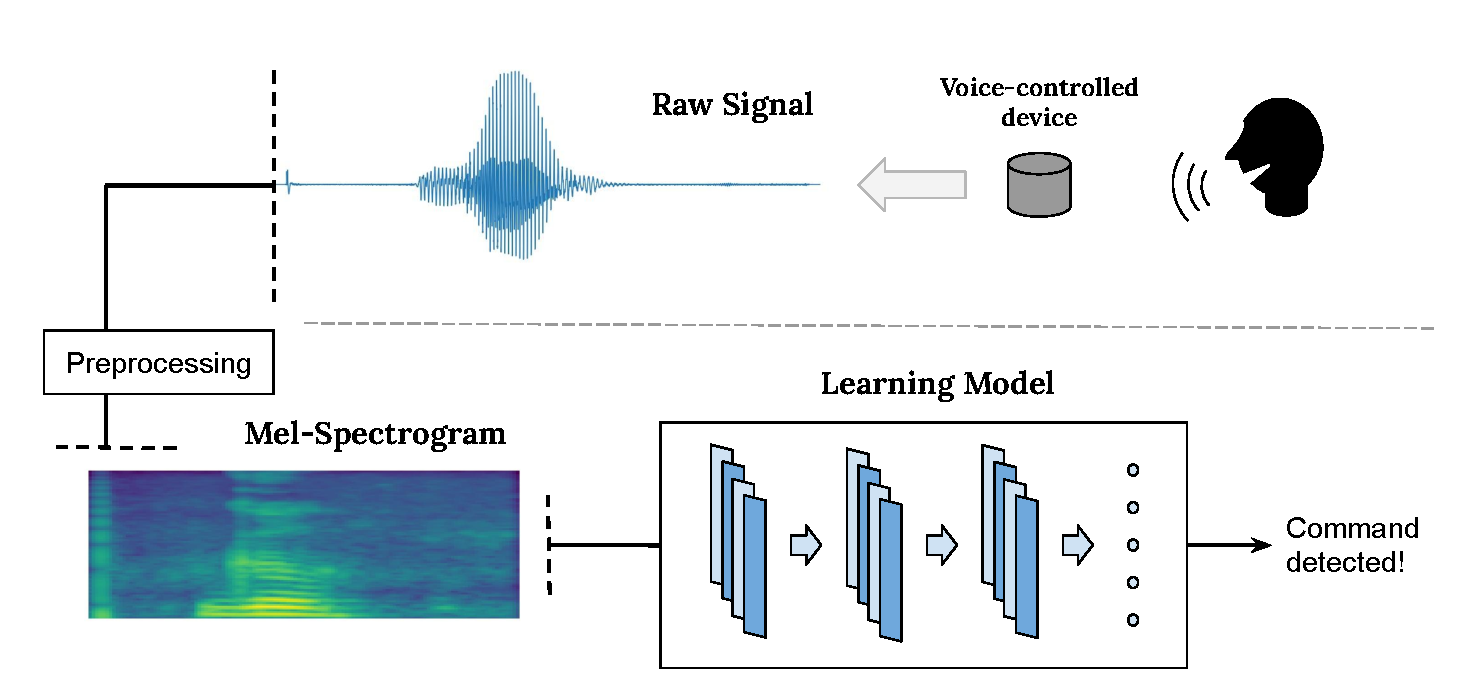
\includegraphics[scale=.35]{processing_pipeline.pdf}}
\caption{Diagram that shows the functioning of voice-controlled devices.}
\label{fig}
\end{figure}
 

The keyword spotting problem that we are trying to solve consists of a multi-class classification task with 12 classes. In particular, 10 of these classes correspond to certain words -- namely "Yes", "No", "Up", "Down", "Left", "Right", "On", "Off", "Stop", and "Go" -- while the remaining 2 are reserved for silence and unknown words.
The dataset that we used (available at \cite{5} and described in \cite{4}), consists of one-second WAV files, for a total of 35 classes plus some additional audio files containing only background noise, from which it is possible to identify the silence samples.


Each audio sample in the train set, validation set, and test set is initially processed in order to extract the audio features, that in our case consist of the Mel-scale spectrogram, and the resulting dataset is cached as a TensorFlow dataset in order to speed up the computations.
These cached versions of the preprocessed dataset are then later used to train and evaluate 2 different classes of models: the first is based on the recurrent neural networks with the attention and the second based on the residual neural network architecture.


Our recurrent neural network implementation was initially inspired by the model described in \cite{1}. 
We improved the first convolutional layers that perform the extraction of local relations by modifying the kernel size and adopting a higher stride in order to keep a meaningful representation, while reducing the number of parameters downstream in the subsequent layers. The core of their implementation is the use of 2 bidirectional LSTM layers from which the attention weight is computed and then used to filter out or boost some components of the LSTM layer output.
Since we are looking for low footprint and high accuracy models we decided to swap these LSTM layers for GRU layers.
Another substantial change is the addition of regularization layers, both in the form of batch normalization layers and dropout layers (spatial dropout when dealing with two-dimensional data). These kinds of changes do not provide a problem in terms of model weight, since they could potentially only slow down the process of training, and do not impact the end devices in any way.


Our residual neural network implementation is based on models described in \cite{2}.
In our implementation, we used a combination of two residual blocks. A first block is a standard residual block that applies an identity function to the input. The second block is described in \cite{14}, where learnable parameters are added to the skip connection, in order to create a nonlinear connection. This technique is useful to reduce the dimensionality of the input for the subsequent layers.
A substantial change is the way in which we organize layers in the residual blocks. In fact, after each convolution layer follows a batch normalization layer and a ReLU activation unit. We also do not use convolution dilation in our models.


In order to maintain small the number of parameters of our models, we tried to keep the number of feature maps low, but without decreasing the performance of the model.
As in \cite{2}, we reduce the size of the input for the final fully connected layer, using a Reduce Mean layer instead of an Average pooling layer.
We noticed that this type of implementation is capable of learning the useful structures of the Mel-Spectrogram, speeding up the learning and also regularizing the model.

\section{Signals and Features}
\label{sec:model}

As mentioned in the Processing Pipeline, the dataset provided by \cite{5} is composed of one-second WAV files, for a total of 35 classes. We adopted the same train-validation-test split that comes with the dataset (80-10-10) and used the test set provided separately \cite{6} that also contains already separated silence samples and a single class called "Unknown" containing a mixture of samples from the classes that we do not care to identify.
This test set contains a similar amount of samples for each of the 12 classes, a ratio that obviously doesn't reflect the classes distribution in the training set that is characterized by an abundance of samples labeled as unknown (25 classes of the entire dataset are actually labeled as unknown, while all the other 10 are taken individually). We solved this distribution problem by filtering randomly, at each training epoch, a suited amount of "Unknown" samples in order to train with the right proportions among all the classes, and to use the entire dataset available.


Since audio samples are usually never fed to a neural network as raw audio files, we tried to explore two common methods for extracting audio features: the Mel-scale spectrogram, and the Mel-frequency cepstral coefficients.
The Mel-scale spectrogram consists of performing the Fast Fourier Transform on overlapping windowed segments of the audio signal. The resulting frequencies are then converted by using the Mel-scale that mimics the sensitivity of the human ear for the different frequencies. Usually the final Mel-Spectrogram is computed by taking the logarithm of the previous values.
The MFCCs are the result of even further processing of the Mel-scale spectrogram. These kinds of features are obtained by applying an additional DCT and eventually selecting a certain number of coefficients.
After some initial tests, we realized that the first method yielded better results, using models of similar size, even when trying different numbers of MFCCs and changing the other preprocessing parameters. This is probably because of the more correlated structure -- also in frequency -- of the features extracted using the Mel-Spectrogram and the fact that neural networks usually work better with rich and more complex representations of the input samples, opposed to imposed and over-processed features as it happens by computing the MFCCs.


Our preprocessing is done by using the Librosa library \cite{7} that provides built-in functions for computing both Mel-Spectrograms and MFCCs. The audio sample is first normalized and then a feature map that consists of an 80-band Mel-scale and 126 time samples, using a 1024 discrete Fourier transform. As neural network input we use the log of the Mel-Spectrogram normalized again.


\section{Learning Framework}
\label{sec:learning_framework}

In this paper we explore two different kinds of architectures and evaluate the tradeoff of different models between accuracy and number of the model parameters. These two families of learning models are attention-based recurrent neural networks and residual neural networks.
The models are implemented by using a high-level API called Keras, based on the TensorFlow library.
Each model is trained similarly, by the use of Adam optimizer \cite{8} for at most 40 epochs. We decided to use the early stopping technique that terminates learning after 10 epochs in which the validation loss does not decrease, and then select the best performing model found during training. Since the problem consists of a multiclass classification we used the sparse categorical cross-entropy loss.
The learning rate follows a custom schedule: it starts from 0.01 and it is decreased by a factor of 0.4 every 15 epochs. The training is divided into batches of 32 samples. As previously mentioned, the dataset is preprocessed by extracting the audio features, then it is cached and at each epoch filtered in order to train with a balanced proportion between all the classes that resemble the one in the test set.



\subsection{Attention-based recurrent neural networks} 
In this section we will describe 4 models that are based on the recurrent neural networks that use attention. We will start by describing the lightest model and then we will underline the changes between the bigger models.

\begin{figure*}[htbp]
\centerline{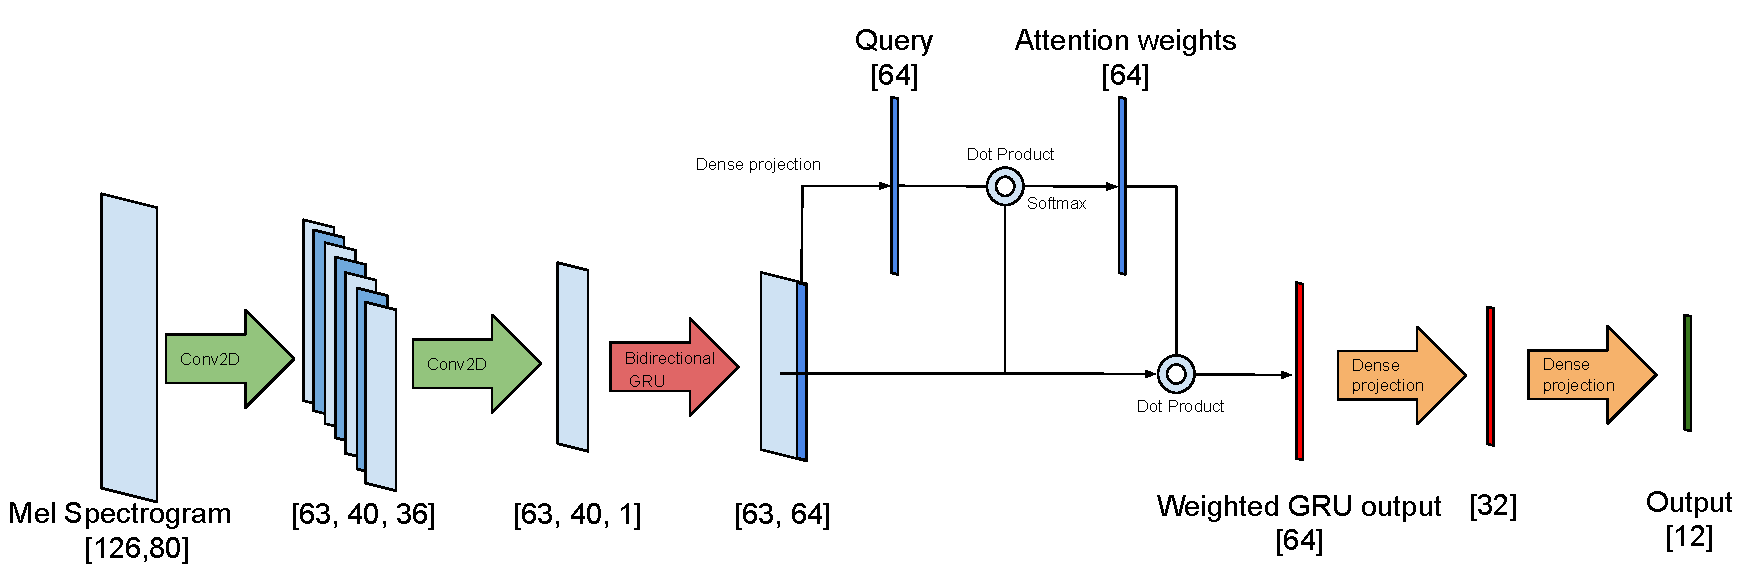
\includegraphics[scale=.5]{att.pdf}}
\caption{Att25K model architecture.}
\label{fig}
\end{figure*}

Our lightest attention model is Att25K, and it requires only 25K parameters. It features two convolutional layers, the first with 32 filters and the second with 1, both with kernel size 3x3. 
These convolutional filters, other than reducing the dimensionality of the input -- since the first convolutional layer has stride equals  2 -- are used to extract local dependency both in frequency and time from the original Mel-Spectrogram.
After each convolution, the ReLU activation function is used and both spatial dropout and batch normalization techniques are deployed for regularization purposes. The second convolutional layer has only one filter in order to effectively be managed by the following bidirectional GRU layer that counts 32 units per direction. 
The output of this recurrent layer is used for computing the attention weights. This is done by taking a dense projection of a single output vector from this layer -- in our case the last one -- and this produces the query. Subsequently, by performing the dot product between the query and the actual output of the GRU layer and taking the softmax, the attention weights are found. The GRU layer output is then filtered by these weights thanks to a dot product. The computation follows 3 fully connected layers for the final classification; the first two use the ReLU activation function, while at the last one the softmax is applied. In order to better generalize the models a dropout layer and a batch normalization layer are used in between each dense layer.
Most of the model parameters are used in the bidirectional GRU layer, which is the main component of our model.
The other attention-based models that we propose have a similar structure and are called: Att50K, Att87K, and Att155K. They have respectively 50, 87, and 155 thousands of parameters.
\begin{itemize}
  \item Att50K features an additional convolutional layer at the beginning with the same parameters of the first one in Att25K, and two GRU layers with 32 units per direction, instead of one.
  \item Att87K has the same initial convolutional layers as Att50K, but a single bidirectional GRU layer with double the parameters, and an additional dense layer for the classification, with 128 neurons.
  \item Att155K is characterized by double the filters in the second convolutional layer with respect to Att87K and two GRU layers with the same parameters.

\end{itemize}
The advantage of using the attention mechanism -- other than being a valuable solution that provides high accuracy -- is that it can easily allow us to visualize, by plotting the attention weights, the most crucial parts in the sample, which determined the final decision as shown in \cite{1}.


  
\subsection{Residual neural networks}
In this section we will describe 4 models that are based on the residual neural network.
We will start by describing the model that in our opinion offers the best tradeoff between accuracy and number of parameters for this kind of architecture.
Subsequently in the section, we will describe all the other models, underlining the substantial differences between them.

\begin{figure*}[htbp]
\centerline{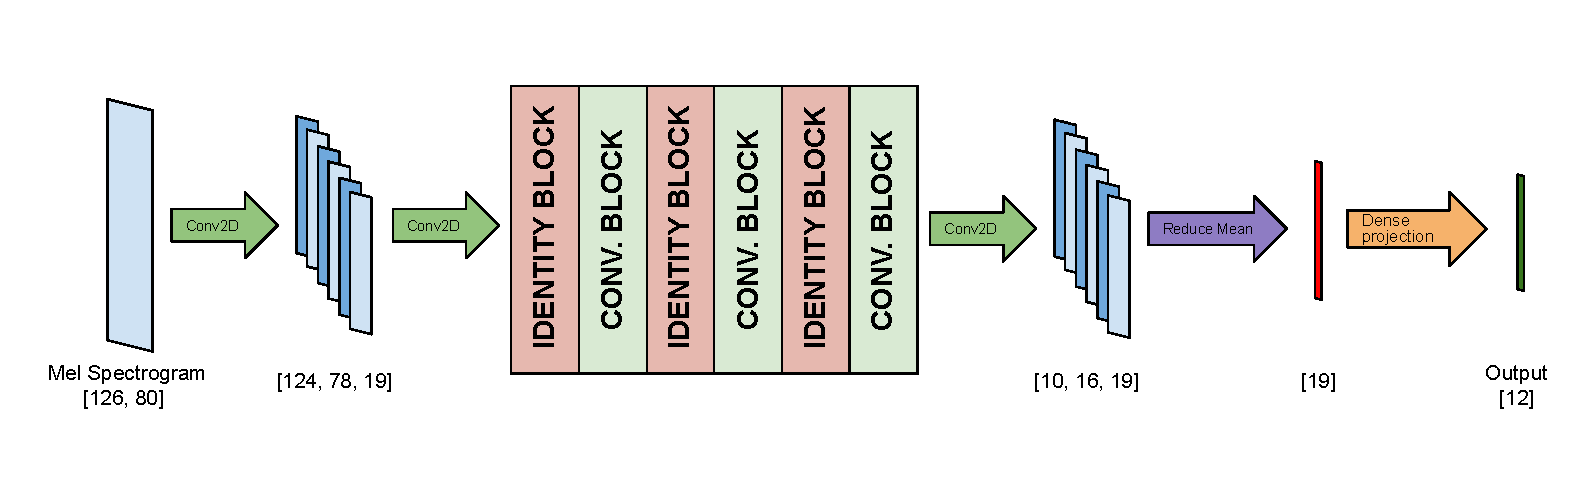
\includegraphics[scale=.6]{res.pdf}}
\caption{Res15narrow model architecture.}
\label{fig}
\end{figure*}

Our best residual model is Res15narrow, which requires 53K parameters.
It is composed of a first convolution layer with 19 filters and kernel size 3x3, followed by a ReLU activation layer and -- instead of dropout -- a batch normalization layer. 
The model proceeds with six residual blocks, starting with an identity residual block, and alternating an identity block with a convolution block.
\begin{figure*}[htbp]
\centerline{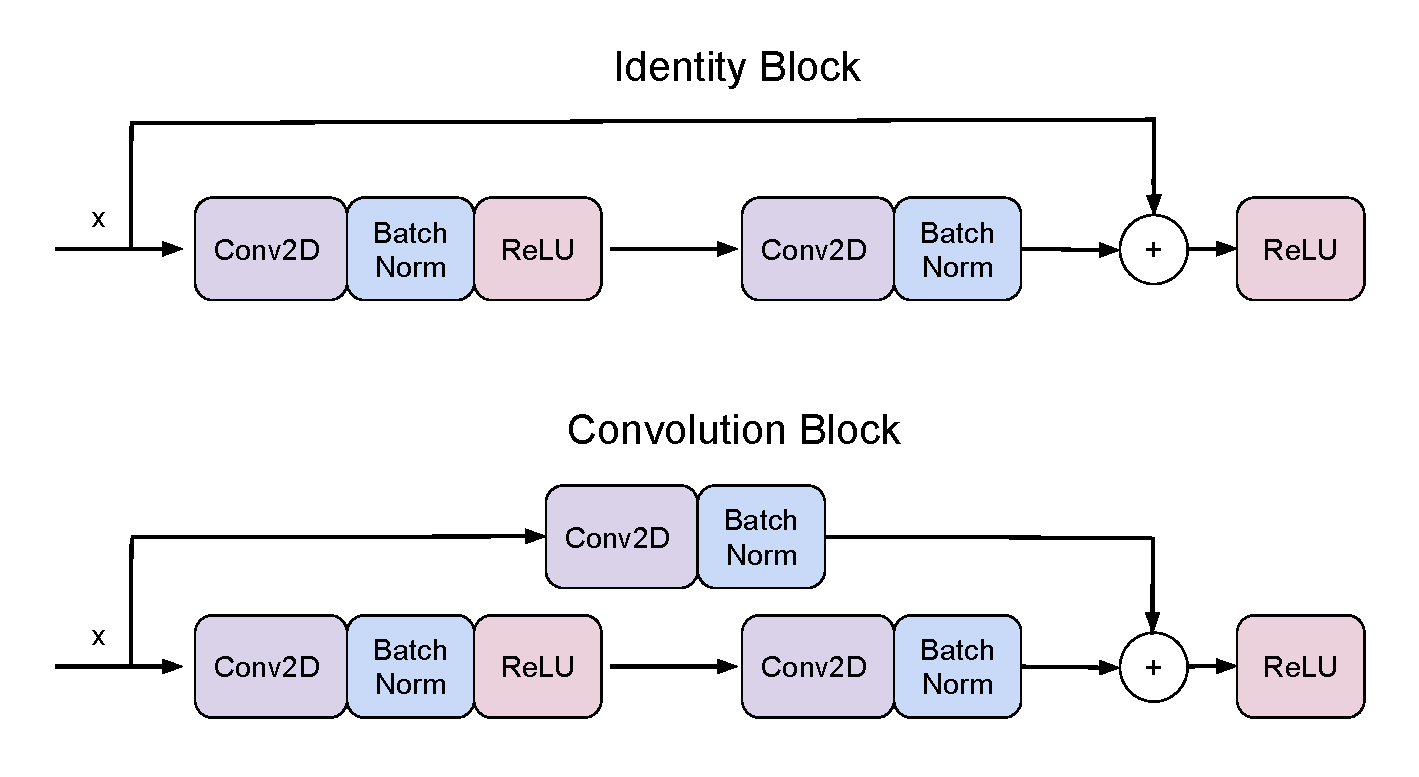
\includegraphics[scale=.47]{res_blocks.pdf}}
\centerline{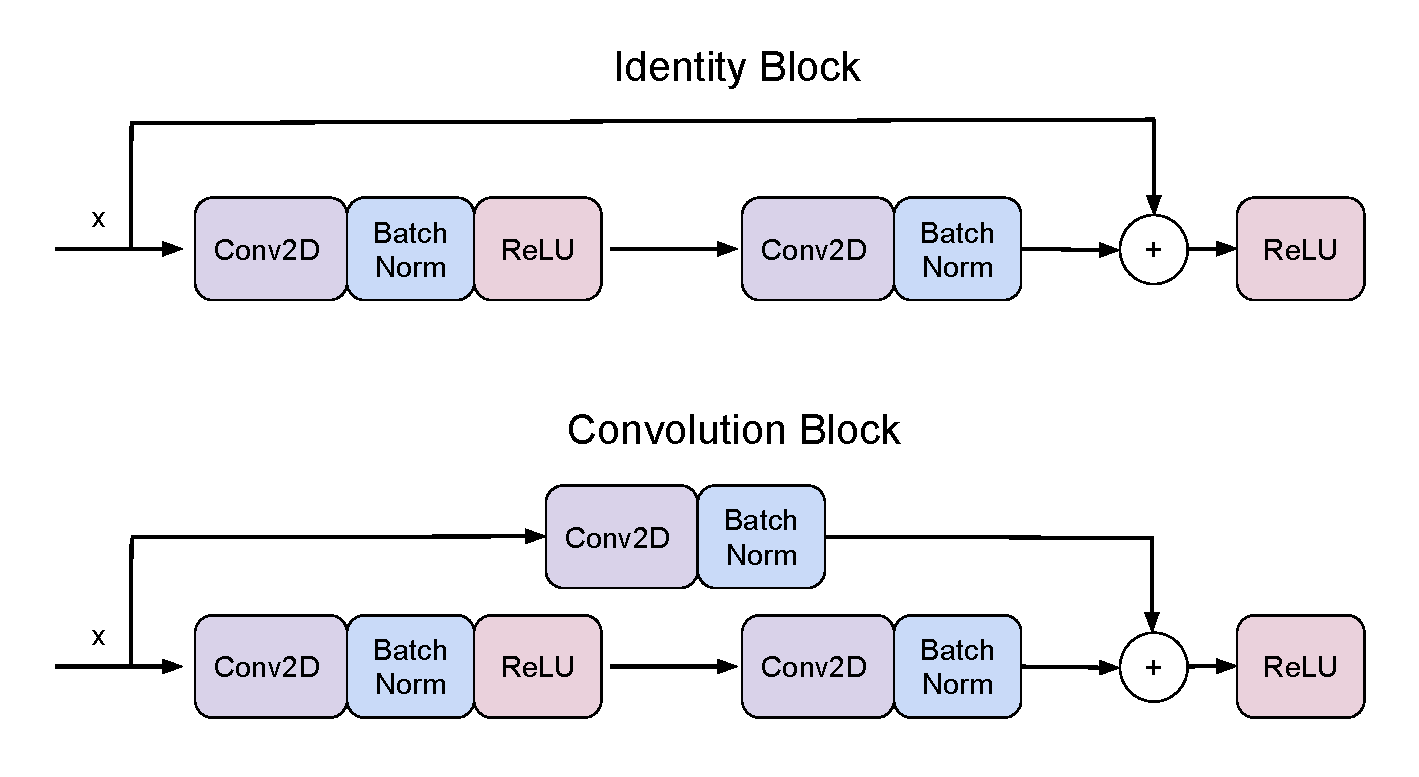
\includegraphics[scale=.47]{Identity_Conv_blocks.pdf}}
\caption{Details of the Identity and Convolution blocks.}
\label{fig}
\end{figure*}
The identity block is composed of two convolution layers with 19 filters and kernel size 3x3. The first one is followed by a batch normalization layer and a ReLU activation layer. The second convolution layer is followed by only a batch normalization layer. At the beginning of the block, the original input is stored, and will be added to the output of the two convolution layers. After the summation, a ReLU activation layer closes the block.
The convolution block is similar, but with the difference that the first convolution block has strides = 2. This is used to reduce the dimensionality of the input while extracting local dependency from the original Mel-Spectrogram.
In this case, in order to preserve the same dimensionality between input and output -- needed to add them together -- we apply to the original input a convolution block with 19 filters, kernel size 3x3 and strides = 2.
A separate non-residual convolution layer and batch normalization layer are further appended to the chain of residual blocks. Instead of a standard Average pooling 2D, a Reduce Mean is used to drastically reduce the dimensionality of the input, that at this point is [10, 16, 19]. The Reduce Mean computes the mean between all the values for each filter, returning a vector of size 19. The latter is fed to a softmax fully connected layer for the final classification.
Almost all of the parameters are equally distributed inside the multiple convolutional layers, leading the network to be quite deep, while keeping the number of parameters rather small.
The other res-net models that we propose have a similar structure and are called: Res8narrow, Res26narrow, and Res8lite. They have respectively 23.4, 92.4, and 57 thousands of parameters.
\begin{itemize}
  \item Res8narrow is composed of a first convolution layer, followed by a 2D average pooling with a 3x4 pool size, thus reducing its output both in time and frequency.
The number of residual blocks is halved (3) compared to Res15narrow, obtaining a very compact model.

  \item Res26narrow has the same initial structure as Res8narrow, that is, a convolution layer followed by an average pooling layer but with size 2x2. 
In this model the number of residual blocks is doubled (12) with respect to Res15narrow, obtaining a deeper model.

  \item Res8lite is characterized, after an initial convolution layer, by a convolution residual block followed by two identity residual blocks. The main difference from other models is that we used 30 filters in each convolution layer instead of 19. 

\end{itemize}
All models end with a Reduce Mean layer, followed by a softmax fully connected layer for the final classification.
We noticed, after some tests, that the final Reduce Mean layer is very useful: not only it  reduces the final input size, but it also functions as a regularizer. We also noticed that dropout layers are not very useful with our models, since they only degrade the performance of the model.



% !TEX root = template.tex

\section{Results}
\label{sec:results}

In this section we will evaluate the performance of our new models in terms of accuracy with respect to the number of parameters that characterize each model. We will also compare our findings with previous state-of-the-art results.

\begin{figure}[htbp]
\centerline{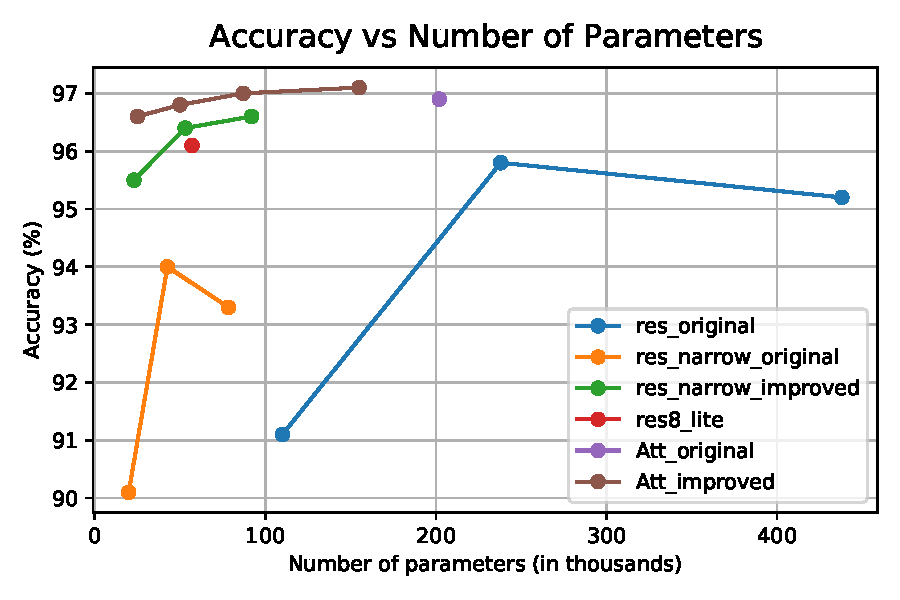
\includegraphics[scale=.6]{acc_vs_par.pdf}}
\caption{Comparison of the accuracy and number of parameters between ours and previous models.}
\label{avp}
\end{figure}

In Figure \ref{avp} we can see a comparison between our new models and the most promising models in the literature. The models we presented are refered to Att\_improved in brown, res\_narrow\_improved in green and res8\_lite in red.
It is clear that our new models bring a noticeable improvement: our enhanced recurrent neural network models based on the attention obtain similar accuracy results as in [1], while having only a fraction (up to 8 times less) of the parameters. The models Att87K and Att155K even slightly surpass the highest accuracy obtained up to now, that was 96.9\% in [1]. In fact, our models obtained respectively 97\% and 97.18\% while having fewer parameters. 
Our res-net models can achieve at least 2\% higher accuracy than the models presented in [2]. However in this case it is worth noting that in [2] they used an older version of the dataset, and different feature extraction (MFCCs as opposed to Mel-Spectrogram). Overall from our tests it seems that our improved implementation of the attention-based recurrent neural networks provides better models: they obtain high accuracy even with limited amounts of parameters. However even our res-net models obtain satisfying levels of accuracy, and can provide a good alternative.

%\begin{figure*}[!htb]
%    \begin{minipage}[t]{.5\textwidth}
%        \centering
%        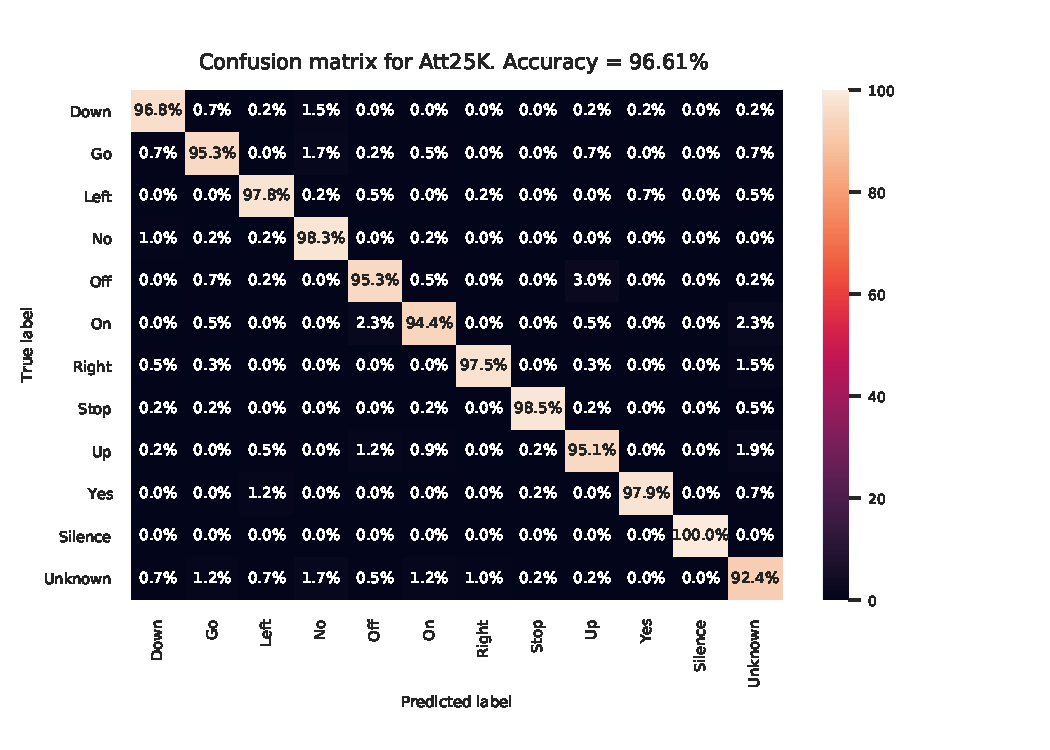
\includegraphics[width=1.1\textwidth]{conf_att.pdf}
%        \subcaption{Image 1.}\label{fig:1}
%    \end{minipage}
%    \hfill
%    \begin{minipage}[t]{.5\textwidth}
%        \centering
%        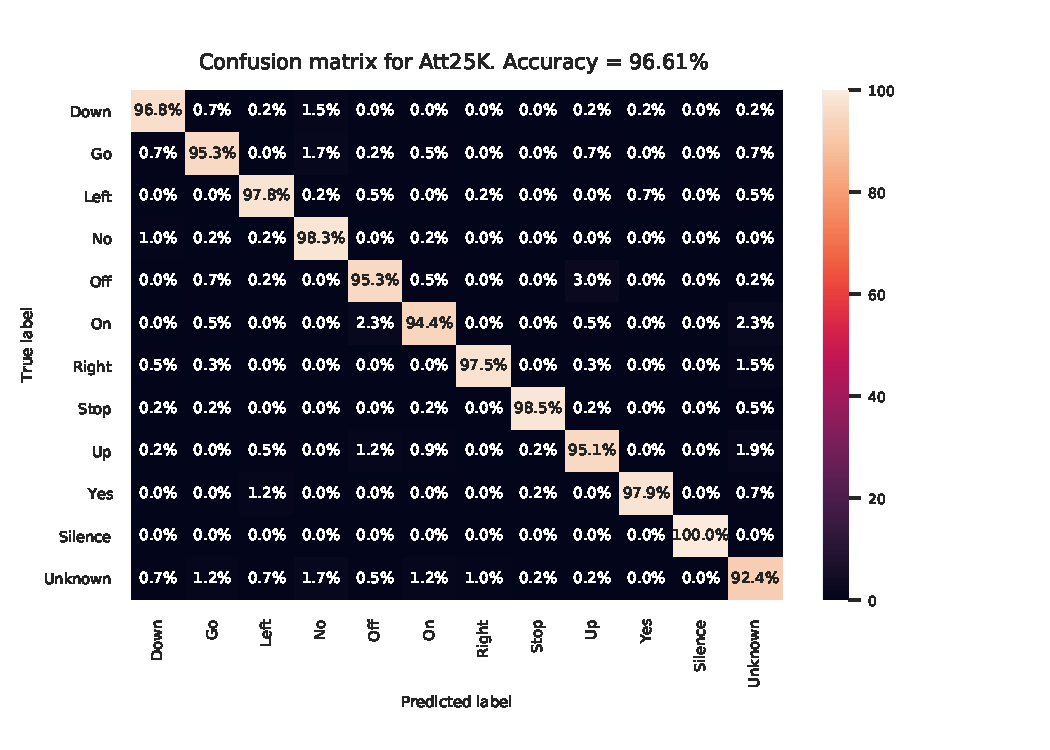
\includegraphics[width=1.1\textwidth]{conf_att.pdf}
%        \subcaption{Image 2.}\label{fig:2}
%    \end{minipage}  
%    \label{fig:1-2}
%    \caption{Title.}
%\end{figure*}

\begin{figure}[htbp]
\centerline{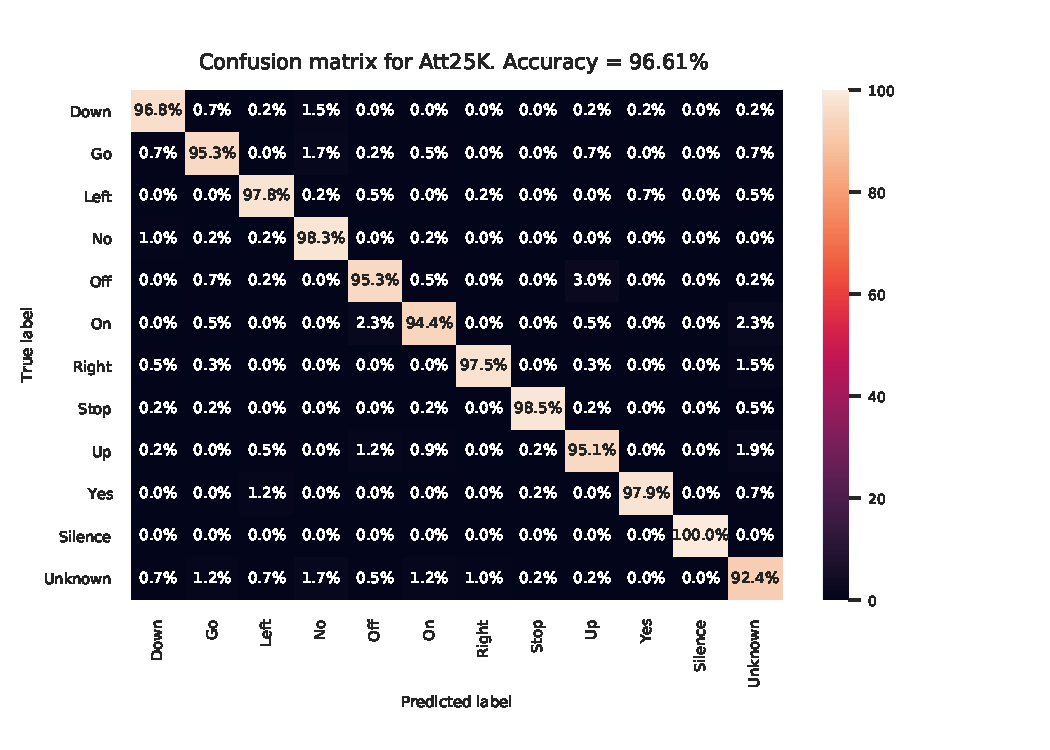
\includegraphics[scale=.5]{conf_att.pdf}}
\caption{Att25K confusion matrix.}
\label{conf_att}
\end{figure}

\begin{figure}[htbp]
\centerline{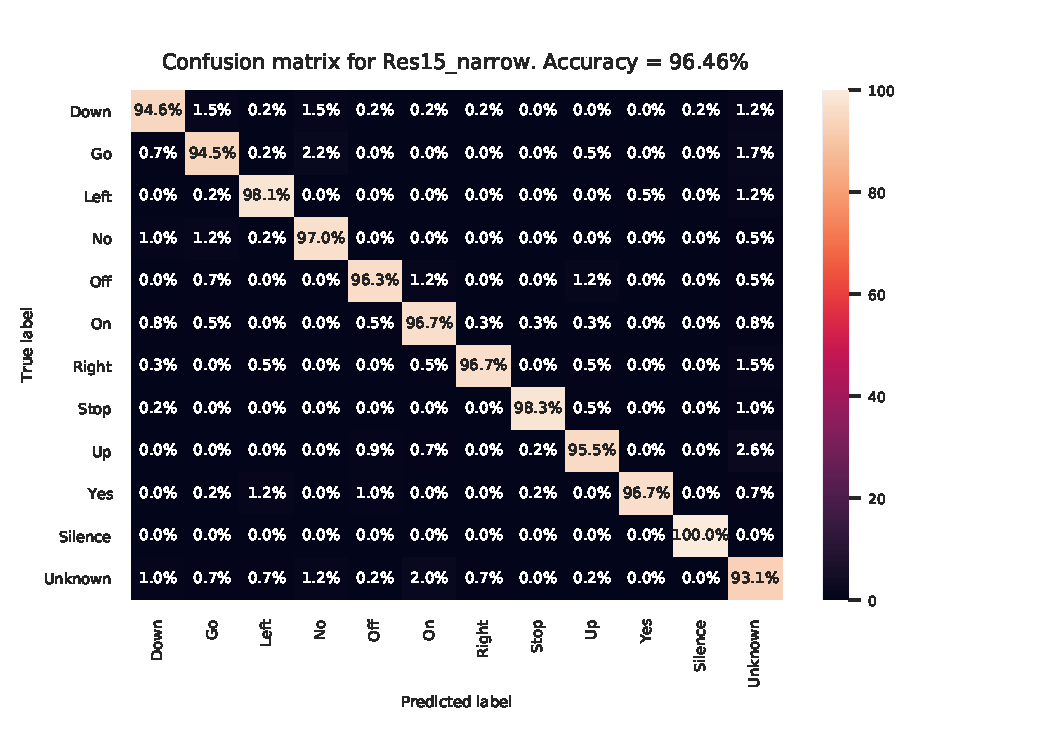
\includegraphics[scale=.5]{conf_res.pdf}}
\caption{Res15\_narrow confusion matrix.}
\label{conf_res}
\end{figure}


In Figures \ref{conf_att} and \ref{conf_res} we provide the confusion matrix of our most interesting models, that are Att25K and Res15narrow. Even if it doesn't offer the best accuracy, Att25K is still reasonably accurate (96.6\%) and it only needs a small number of parameters.
Res15narrow represents a good tradeoff, for what concerns the residual-based models, between the number of parameters and accuracy, even if it has more than double the parameters of Att25K.
From both the confusion matrices we can notice that the hardest class to manage is the "Unknown" class.
For that class the accuracy is, respectively, 92.4\% and 93\%, which is low compared to the other classes. We noticed that sometimes unknown samples are interpreted as actual commands, and at the same time some commands are not recognized as such and are classified as unknown words. Another problematic pair of classes that are sometimes misclassified with each other are "on" and "off". For the opposite meaning that these two commands have, this can actually be a relevant problem in a final application and would need further addressing.


\begin{figure}[htbp]
\centerline{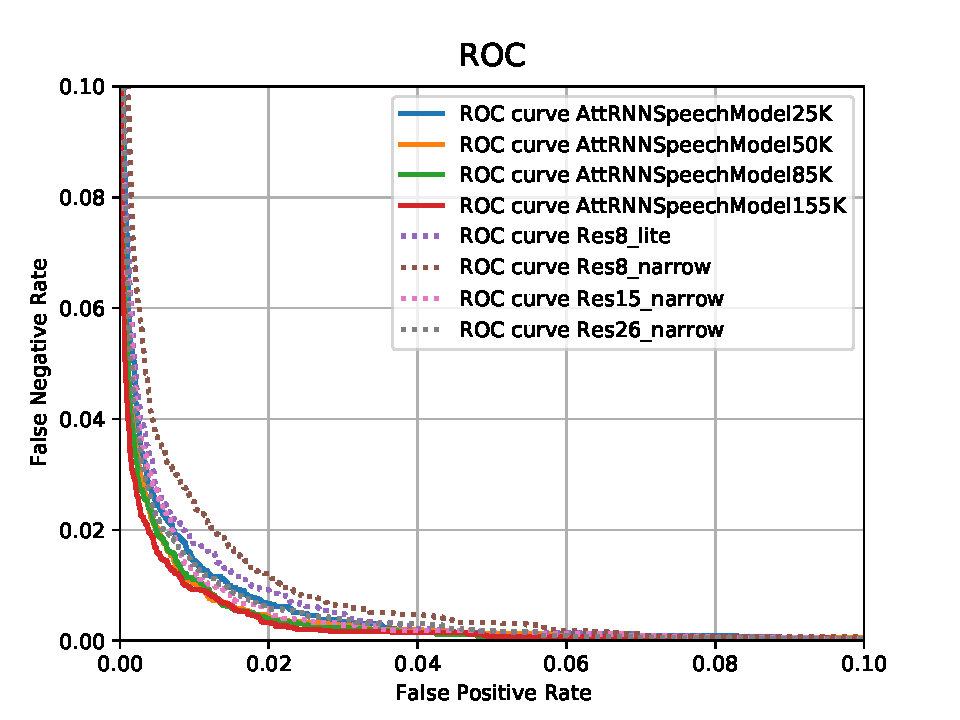
\includegraphics[scale=.5]{ROC.pdf}}
\caption{ROC curves for the different models.}
\label{roc}
\end{figure}

In order to further compare our new models, we show the receiver operating characteristic (ROC) curves. In Figure \ref{roc} the x-axis represents the false-positive rate, while the y-axis shows the false-negative rate, and each point of the curve is computed by considering a different threshold. Every curve corresponds to a single model and it is computed by micro averaging all the curves for each class compared with all the other classes. The models that have a smaller area under the corresponding curve are better. We can notice that the curves of our models are almost all comparable.


% !TEX root = template.tex

\section{Concluding Remarks}
\label{sec:conclusions}

In this paper we studied two different architectures: attention-based recurrent neural networks and residual networks. We proposed several models for each architecture, that differ by the number of parameters, but all of them can be considered to have high, and almost comparable, accuracy. Some of our models even outperform the previous state-of-the-art solutions, while having fewer parameters. In particular, our most relevant model, Att25K with only 25K parameters can achieve an accuracy of 96.6\%. Finding small-footprint models that can achieve high accuracy is crucial in order to deploy devices that can mount less expensive and less powerful hardware, while performing the task of keyword spotting for voice control in a reliable way.
In a real-world application we think that smarter management of silence samples would be very useful since most of the time the input recordings are likely to be silence. This should be better done independently from the neural network model, limiting the use of the latter only if the sample detected contained a certain amount of sound.

During this project we learned how to deal with audio samples and how to extract features from them. We explored two important neural network architectures, namely attention-based recurrent neural networks and residual neural networks.
Moreover, we gained a particular sensibility towards the model dimension, and how it is important for some kind of applications to find models that can deliver high accuracy while having a small footprint.


\bibliography{biblio}
\bibliographystyle{ieeetr}

\end{document}


